\begin{center}
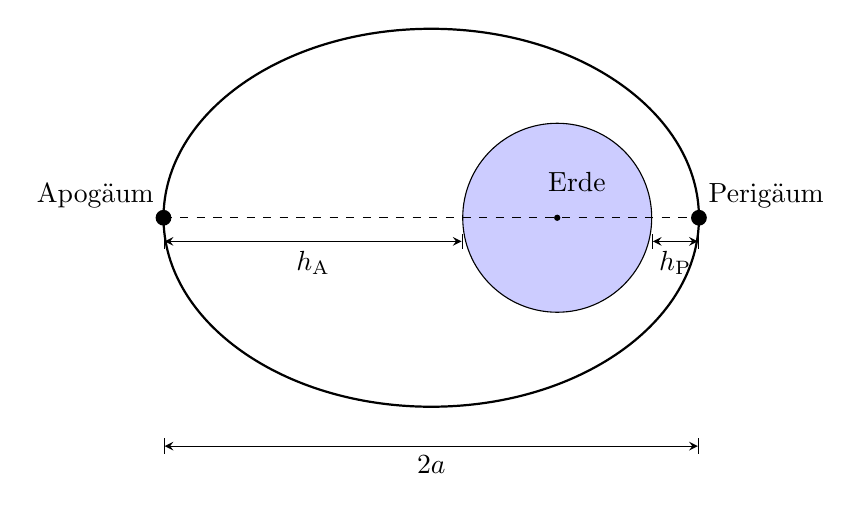
\begin{tikzpicture}[>=stealth]
 \fill[blue!20] (0,0) circle (1.2);
 \draw (0,0) circle (1.2);
 \fill (0,0) circle (0.04);
 \node at (0.25,0.45) {Erde};
 \draw[thick] (-1.6,0) ellipse (3.4 and 2.4);
 \draw[dashed] (-5,0) -- (1.8,0);
 \fill (1.8,0) circle (0.1) node[above right] {Perigäum};
 \fill (-5,0) circle (0.1) node[above left] {Apogäum};
 \draw[|<->|] (1.2,-0.3) -- (1.8,-0.3) node[midway, below] {$h_\mathrm{P}$};
 \draw[|<->|] (-5,-0.3) -- (-1.2,-0.3) node[midway, below] {$h_\mathrm{A}$};
 \draw[|<->|] (-5,-2.9) -- (1.8,-2.9) node[midway, below] {$2a$};
\end{tikzpicture}
\end{center}

Der Erdmittelpunkt liegt in einem Brennpunkt der Bahnellipse. Perigäum und Apogäum liegen sich gegenüber, ihre Abstände vom Erdmittelpunkt ergeben zusammen die grosse Achse:
\begin{align}
 2a &= \left(r_\mathrm{E}+h_\mathrm{P}\right)+\left(r_\mathrm{E}+h_\mathrm{A}\right)
 \quad\Rightarrow\quad a = r_\mathrm{E}+\frac{h_\mathrm{P}+h_\mathrm{A}}{2}
\end{align}
Mit $r_\mathrm{E} = \RErO$ (FoTaBe S.~209):
\begin{align}
 a_\text{Nimbus} &= \REr+\frac{\hpNi+\haNi}{2} = \aNi \approx \result{\aNiP{3}{4}} \\
 a_\text{Skynet} &= \REr+\frac{\hpSk+\haSk}{2} = \aSk \approx \result{\aSkP{3}{4}} \\
 a_\text{Nato} &= \REr+\frac{\hpNa+\haNa}{2} = \aNa \approx \result{\aNaP{3}{4}}
\end{align}
Nach dem dritten Keplerschen Gesetz, das für Ellipsenbahnen mit der grossen Halbachse $a$ gleich lautet wie für Kreisbahnen mit dem Radius $a$, gilt
\begin{align}
 \frac{a^3}{T^2} &= \frac{G\,M_\mathrm{E}}{4\pi^2}
 \quad\Rightarrow\quad M_\mathrm{E} = \frac{4\pi^2 a^3}{G\,T^2}
\end{align}
Damit ergeben die drei Satelliten
\begin{align}
 M_\text{Nimbus} &= \frac{4\pi^2\cdot\left(\aNi\right)^3}{\ncG\cdot\left(\TNi\right)^2} = \MNi \approx \result{\MNiS{3}} \\
 M_\text{Skynet} &= \frac{4\pi^2\cdot\left(\aSk\right)^3}{\ncG\cdot\left(\TSk\right)^2} = \MSk \approx \result{\MSkS{3}} \\
 M_\text{Nato} &= \frac{4\pi^2\cdot\left(\aNa\right)^3}{\ncG\cdot\left(\TNa\right)^2} = \MNa \approx \result{\MNaS{3}}
\end{align}
Der Mittelwert ist $M_\mathrm{E} \approx \result{\MMiS{3}}$, in guter Übereinstimmung mit dem Tabellenwert $\MErO$ (FoTaBe S.~209). Die Abweichungen von einigen Promille kommen von den gerundeten Bahndaten und davon, dass die Erde keine exakte Kugel ist (Äquatorradius \RAeqO).
